\chapter{The ILC Environment}
\label{chap:ilc}
\label{ild:sec:ilc}
%\writer{Karsten Buesser, Keisuke Fujii}{3}

In this chapter the latest status of the International Linear Collider layout and design parameters are summarized, as well as the corresponding experimental conditions for the ILD detector.

\section{The International Linear Collider Project}
The ILC is a high-luminosity linear electron-positron collider based on the 1.3~GHz superconducting RF accelerating technology. The ILC has been initially proposed for an energy range of 200-500~\GeV, upgradable to 1\,TeV~\cite{Behnke:2013xla}. After the discovery of the Higgs Boson at 125~\GeV~mass, the baseline of the ILC has been re-configured with an initial stage at 250~\GeV~ center-of-massenergy~\cite{Bambade:2019fyw}, which provides a rich harvest for a precision Standard Model and Higgs physics programme. The baseline ILC can be extended to higher energies and luminosities in well defined upgrade scenarios. The basic beam parameters for the baseline and potential upgrades are given in table~\ref{tab:ilc-params}.

\begin{table}[tbhp]
\begin{adjustbox}{width=1.\textwidth,center=\textwidth}
\begin{tabular}{lccccccc}
Quantity & Symbol & Unit & Initial & ${\mathcal{L}}$ Upgrade & TDR &  \multicolumn{2}{c}{Upgrades} \\
\hline
Centre of mass energy & $\sqrt{s}$ & ${\mathrm{\GeV}}$ & $250$ & $250$ & $250$ & $500$ & $1000$ \\
Luminosity & \multicolumn{2}{c}{${\mathcal{L}}$ ~~~~$10^{34}{\mathrm{cm^{-2}s^{-1}}}$} & $1.35$ & $2.7$ & $0.82$ & $1.8 / 3.6$ & $4.9$ \\
Polarisation for $e^- (e^+)$ & $P\sub{-} (P\sub{+})$ & & ~$80\,\% (30\,\%)$~ &  ~$80\,\% (30\,\%)$~ &  ~$80\,\% (30\,\%)$~ &~$80\,\% (30\,\%)$~ &  ~$80\,\% (20\,\%)$~  \\
Repetition frequency &$f\sub{{rep}}$ & ${\mathrm{Hz}}$  & $5$ & $5$ & $5$ & $5$ & $4$ \\
Bunches per pulse  &$n\sub{{bunch}}$ & 1  & $1312$ & $2625$ & $1312$ & $1312 / 2625$ & $2450$ \\
Bunch population  &$N\sub{{e}}$ & $10^{10}$ & $2$ &  $2$ & $2$ & $2$ & $1.74$ \\
Linac bunch interval & $\Delta t\sub{{b}}$ & ${\mathrm{ns}}$ & $554$ & $366$ & $554$ & $554 / 366$ & $366$ \\
Beam current in pulse & $I\sub{{pulse}}$ & ${\mathrm{mA}}$& $5.8$ & $5.8$& $8.8$ & $5.8$ & $7.6$  \\
Beam pulse duration  & $t\sub{{pulse}}$ & ${\mathrm{\mu s}}$ & $727$ & $961$ & $727$ & $727 / 961$ & $897$ \\
Average beam power  & $P\sub{{ave}}$   & ${\mathrm{MW}}$ & $5.3$ & $10.5$ & $10.5$ & $10.5 / 21$  & $27.2$ \\  
Norm. hor. emitt. at IP & $\gamma\epsilon\sub{{x}}$ & ${\mathrm{\mu m}}$& $5$ & $5$ & $10$ & $10$ & $10$  \\ 
Norm. vert. emitt. at IP & $\gamma\epsilon\sub{{y}}$ & ${\mathrm{nm}}$ & $35$ & $35$ & $35$ & $35$ & $30$ \\ 
RMS hor. beam size at IP  & $\sigma^*\sub{{x}}$ & ${\mathrm{nm}}$  & $516$ & $516$ & $729$ & $474$ & $335$ \\
RMS vert. beam size at IP &$\sigma^*\sub{{y}}$ & ${\mathrm{nm}}$ & $7.7$  & $7.7$  & $7.7$  & $5.9$ & $2.7$ \\
Luminosity in top $1\,\%$ & ${\mathcal{L}}\sub{0.01} / {\mathcal{L}}$ &  & $73\,\%$  &  $73\,\%$ & $87.1\,\%$  & $58.3\,\%$ & $44.5\,\%$\\
Energy loss from beamstrahlung  & $\delta\sub{BS}$ &  & $2.6\,\%$  & $2.6\,\%$  & $0.97\,\%$  & $4.5\,\%$ & $10.5\,\%$ \\
Site AC power  & $P\sub{{site}}$ &  ${\mathrm{MW}}$ & $129$ & & $122$ & $163$ & $300$ \\
Site length & $L\sub{{site}}$ &  ${\mathrm{km}}$ & $20.5$ & $20.5$ & $31$ & $31$ & $40$ \\
\end{tabular}
\caption{Summary table of the ILC accelerator parameters in the initial 250~\GeV~staged configuration (with TDR parameters at 250~\GeV~given for comparison) and possible upgrades~\cite{Bambade:2019fyw}. A 500~\GeV~machine could also be operated at 250~\GeV~with 10~Hz repetition rate, bringing the maximum luminosity to 5.4$\cdot$10$^{34}$cm$^{-2}$s$^{-1}$~\cite{Harrison:2013nva}.
\label{tab:ilc-params}}
\end{adjustbox}
\end{table}

Recently, options for running the ILC-250 machine at the Z pole have been re-evaluated~\cite{Yokoya:2019rhx}. Luminosities in the order of 2.5 $\times$ 10$^{33}$ cm$^{-2}$s$^{-1}$ are in reach with moderate modifications of the ILC beam parameters. Increasing this value to $\approx$ 5 $\times$ 10$^{33}$ cm$^{-2}$s$^{-1}$ can be realised when the number of bunches per pulse is doubled, as currently suggested for the luminosity upgrade scenarios at higher energies~(c.f.~table~\ref{tab:ilc-params}).

The layout of the baseline 250~\GeV~ILC facility is shown in figure~\ref{ild:fig:ilc_footprint}. The total linear accelerator length is about 20.5~km with an experimental area hosting two detectors in push-pull configuration in the interaction region located at the center. The ILC design foresees a crossing angle of 14~mrad between the linac arms.
\begin{figure}[!ht]
\centering
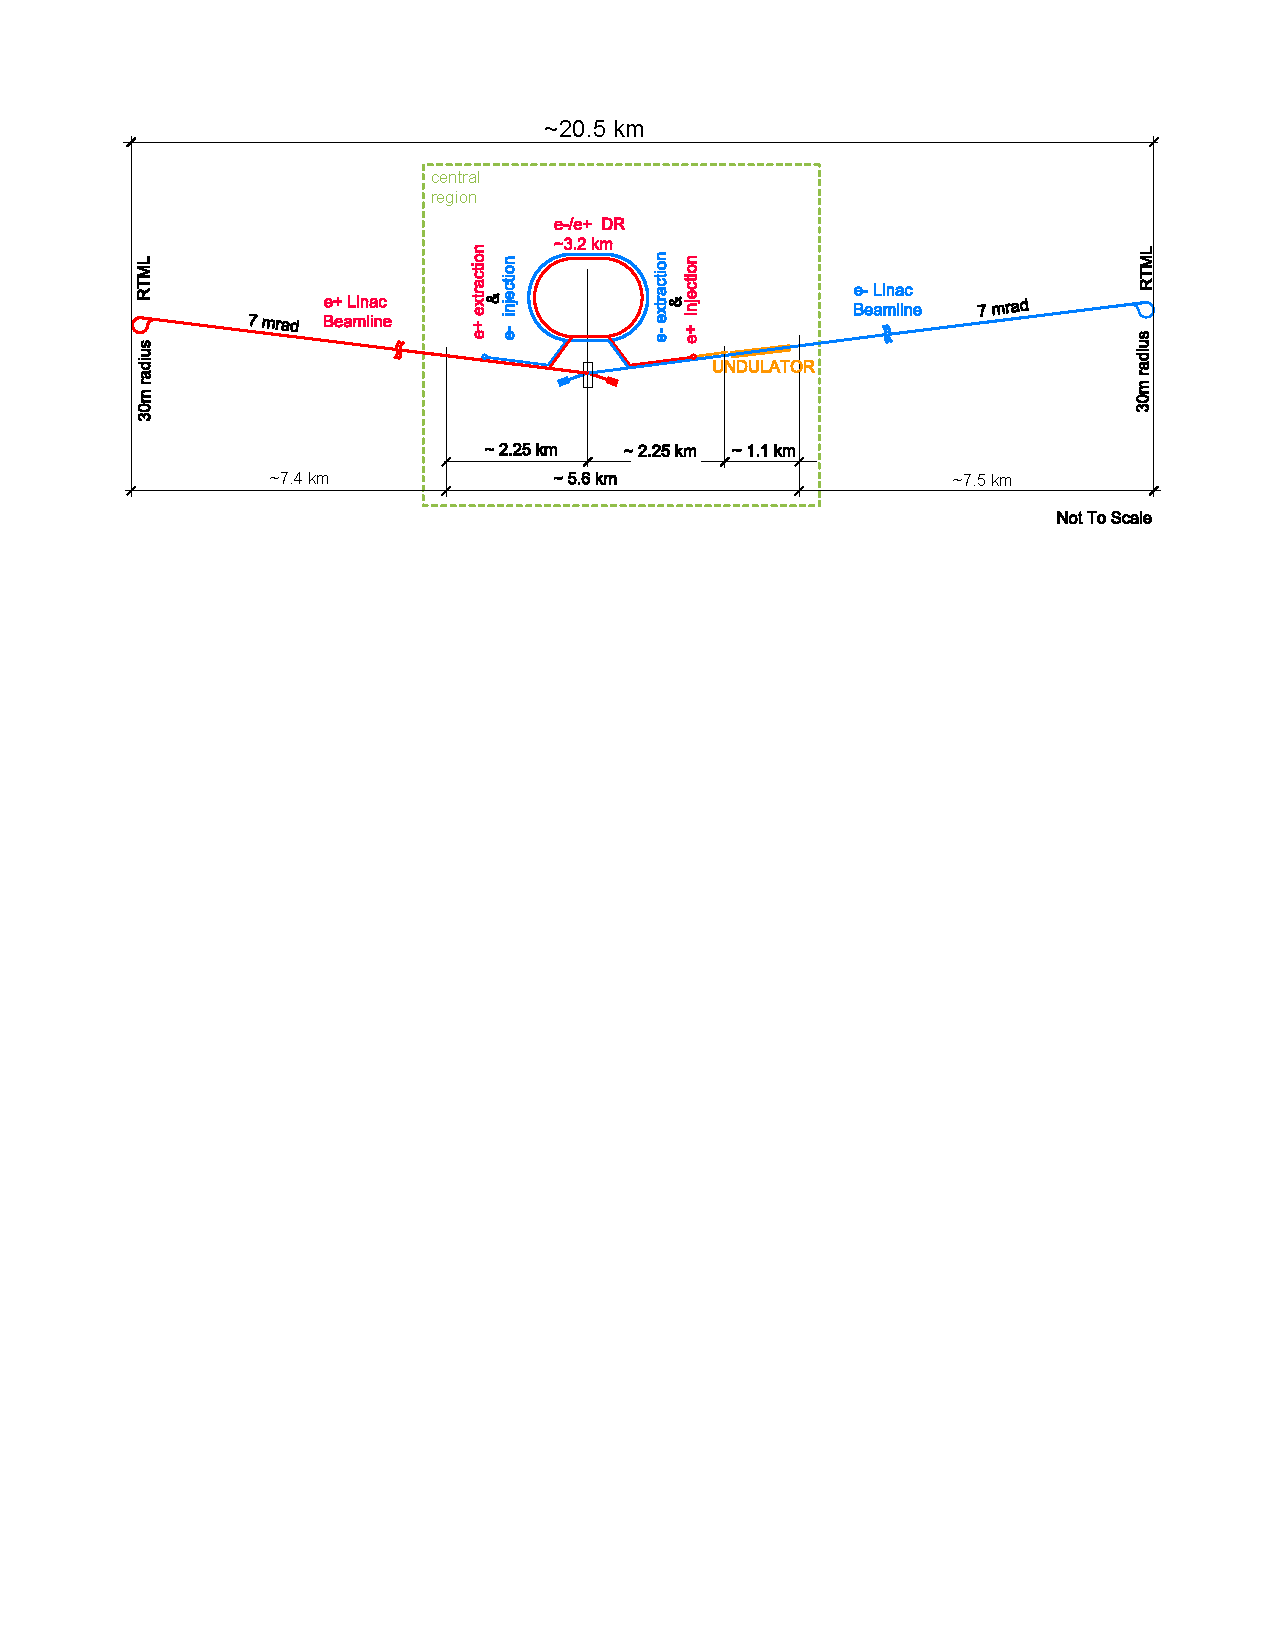
\includegraphics[width=0.9\hsize]{ILC/figs/ILC_Footprint.pdf}

\caption{\label{ild:fig:ilc_footprint}Layout of the ILC in the 250~\GeV~baseline configuration~\cite{Bambade:2019fyw}.}
\end{figure}
The Japan Association of High Energy Physicists (JAHEP) has proposed that Japan hosts the ILC as a staged project~\cite{ild:bib:JAHEP}. A possible site for the construction of the ILC has been idenfitied in the Kitakami mountains in the Tohoku area in the north of Honshu main island, about 400~km north of Tokyo. Figure~\ref{ild:fig:ilc_site} shows the location that allows for a total linac length of about 50~km, and therefore extension space for upgrade scenarios, in good geological conditions. Figure~\ref{ild:fig:ilc_tunnel} shows the cross section of the ILC main linac tunnel with the cryomodules in the right section and the klystrons and RF distribution in the left section.
\begin{figure}[htbp]
\centering
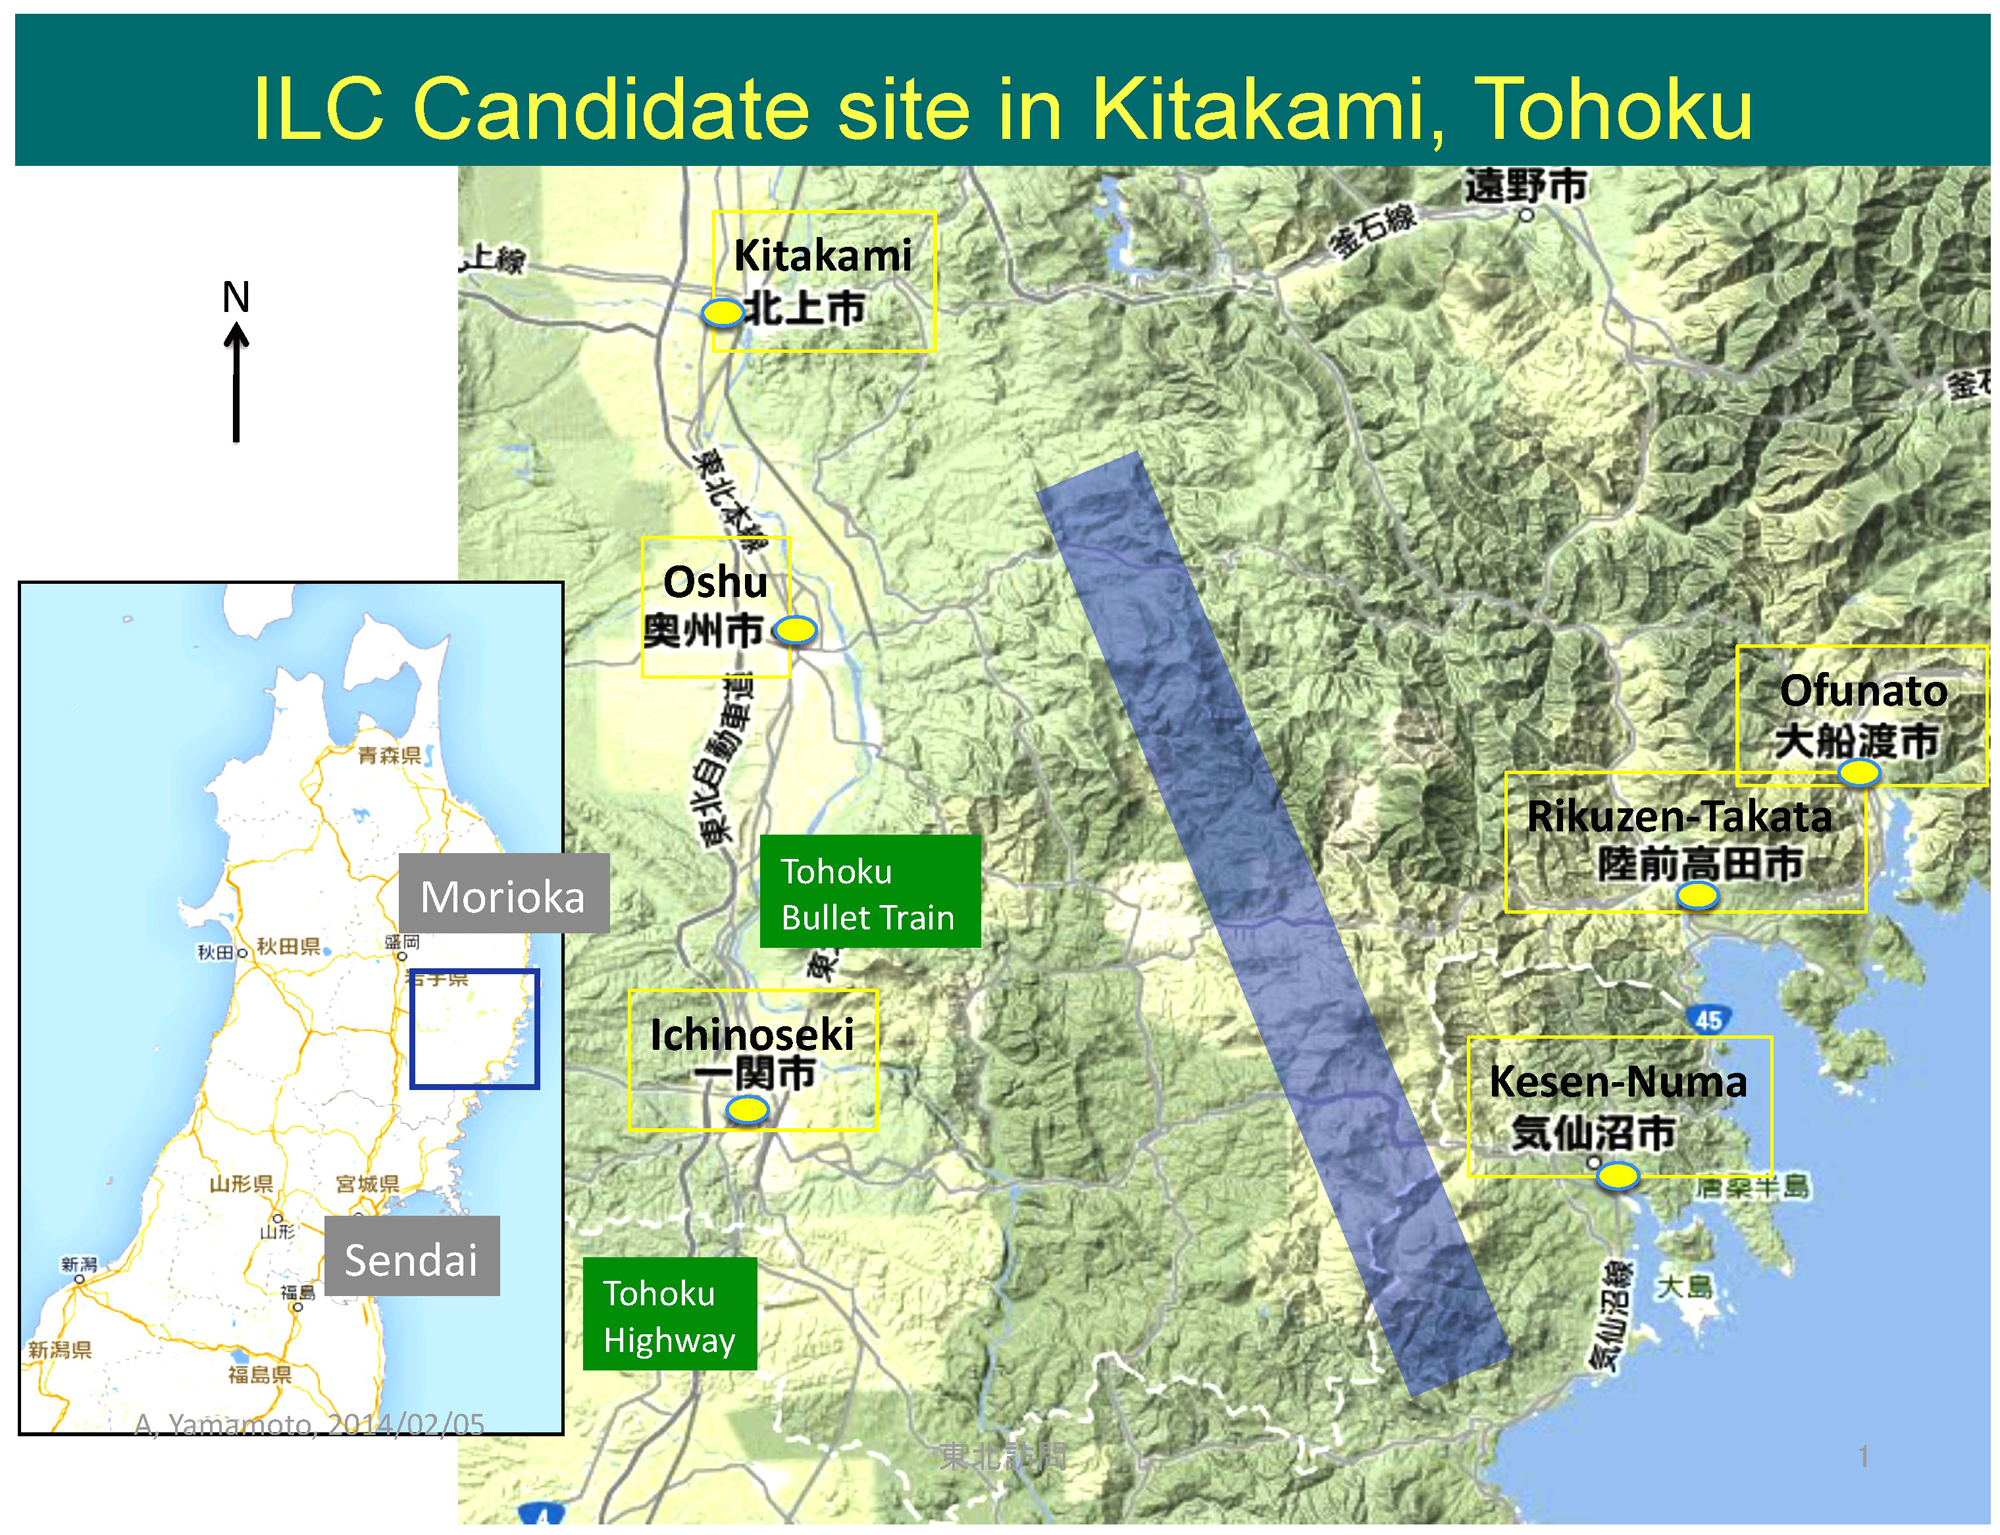
\includegraphics[width=0.9\hsize]{ILC/figs/ILC-Candidate-Area.jpg}
\caption{\label{ild:fig:ilc_site}Location of the ILC candidate site in the Kitakami mountains of Tohoku, Japan~\cite{ild:bib:Newsline_Kitakami}.}
\end{figure}
\begin{figure}[htbp]
\centering
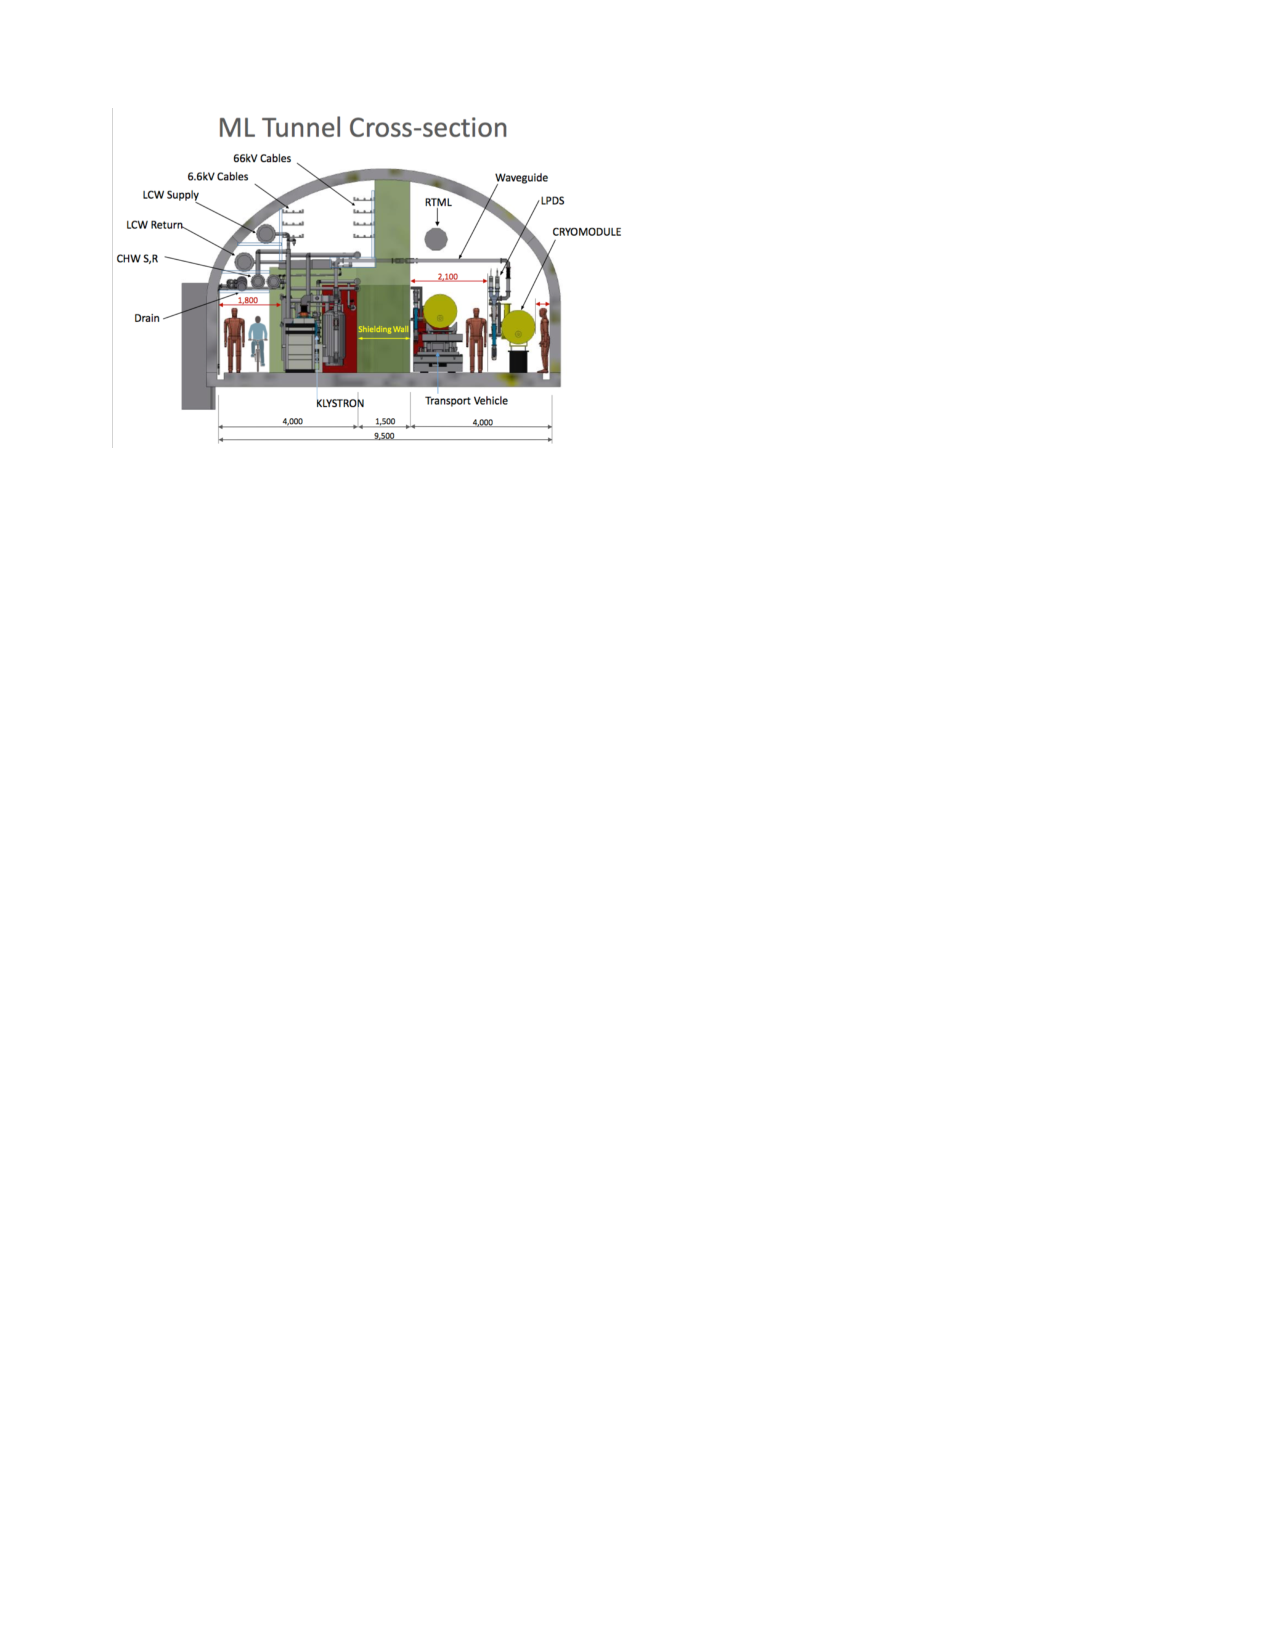
\includegraphics[width=0.8\hsize]{ILC/figs/ilc_tunnel.pdf}
\caption{\label{ild:fig:ilc_tunnel}Cross section of the ILC main linac tunnel~\cite{Bambade:2019fyw}.}
\end{figure}
The specific location of the ILC site and the local conditions, e.g. in terms of street access and topography, has implications on the design, assembly and operations of ILD, as discussed in section~\ref{ild:sec:access}.

\section{Integration of ILD into the experimental environment}
ILD is designed to operate in a push-pull arrangement with another detector, sharing one common ILC interaction region. In this scheme ILD sits on a movable platform in the underground experimental hall. This platform allows for a roll-in of ILD from the parking position into the beam and vice versa within a few hours. The detector can be fully opened and maintained in the parking position.

The current mechanical design of ILD assumes an initial assembly of the detector on the surface, similar to the construction of CMS at the LHC. A vertical shaft from the surface into the underground experimental cavern allows ILD to be lowered in five large segments, corresponding to the five yoke rings.

ILD is designed to fully cope with the ILC beam conditions~(c.f.~Section~\ref{ild:sec:beam_backgrounds}). The expected levels of beam induced backgrounds have been simulated and are seen to be at tolerable levels, {\it e.g.} for the vertex detectors. Judiciously placed shielding keeps scattered backgrounds under control. Regarding the collider, the design of the interaction region and the collimation system has been defined so as to keep the external background sources at levels below the detector requirements.

ILD is self-shielding with respect to radiation and magnetic fields to enable the operation and maintenance of equipment surrounding the detector, {\it e.g.} cryogenics. Of paramount importance is the possibility to operate and maintain the second ILC push-pull detector in the underground cavern during ILC operation~(c.f.~Section~\ref{ild:sec:external_integration}).

\section{Experimental Conditions}
 
\subsection{Beam Conditions} \label{sec:beam:conditions}
The ILC beams have specific properties that are optimised for the physics output of the experimental programme:
\begin{itemize}
\item High instantaneous luminosity: 1.35$\cdot$10$^{34}$cm$^{-2}$s$^{-1}$ at $\sqrt{s}=$250~\GeV cms;
\item Longitudinal polarisation for the electron (80\%) and positron (30\%) beams;
\item Moderate energy losses from beamstrahlung;
\item A pulse structure with pulse lengths of $\approx$ 1~ms and low repetition rates of 5-10~Hz which enables the use of power-pulsed readout schemes in the detector.
\item A beam crossing angle of 14 mrad at the collision point.
\end{itemize}
To reach high luminosities, the ILC bunches are focused to very small cross sections in the nanometre range at the interaction point (see Table~\ref{tab:ilc-params}). The new baseline ILC-250 was optimised for maximum luminosity with an increased beam focusing compared to the TDR, resulting in a slightly increased beam energy spread for interactions. The luminosity spectrum describes the distribution of the luminosity versus the centre-of-mass energy. Figure~\ref{fig:ilc:ecmspect-250} shows the luminosity spectrum for ILC-250, Figure~\ref{fig:ilc:ecmspect-500} for the 500~\GeV~upgrade.

\begin{figure}[htbp]
%\begin{center}
\begin{subfigure}{0.49\hsize} 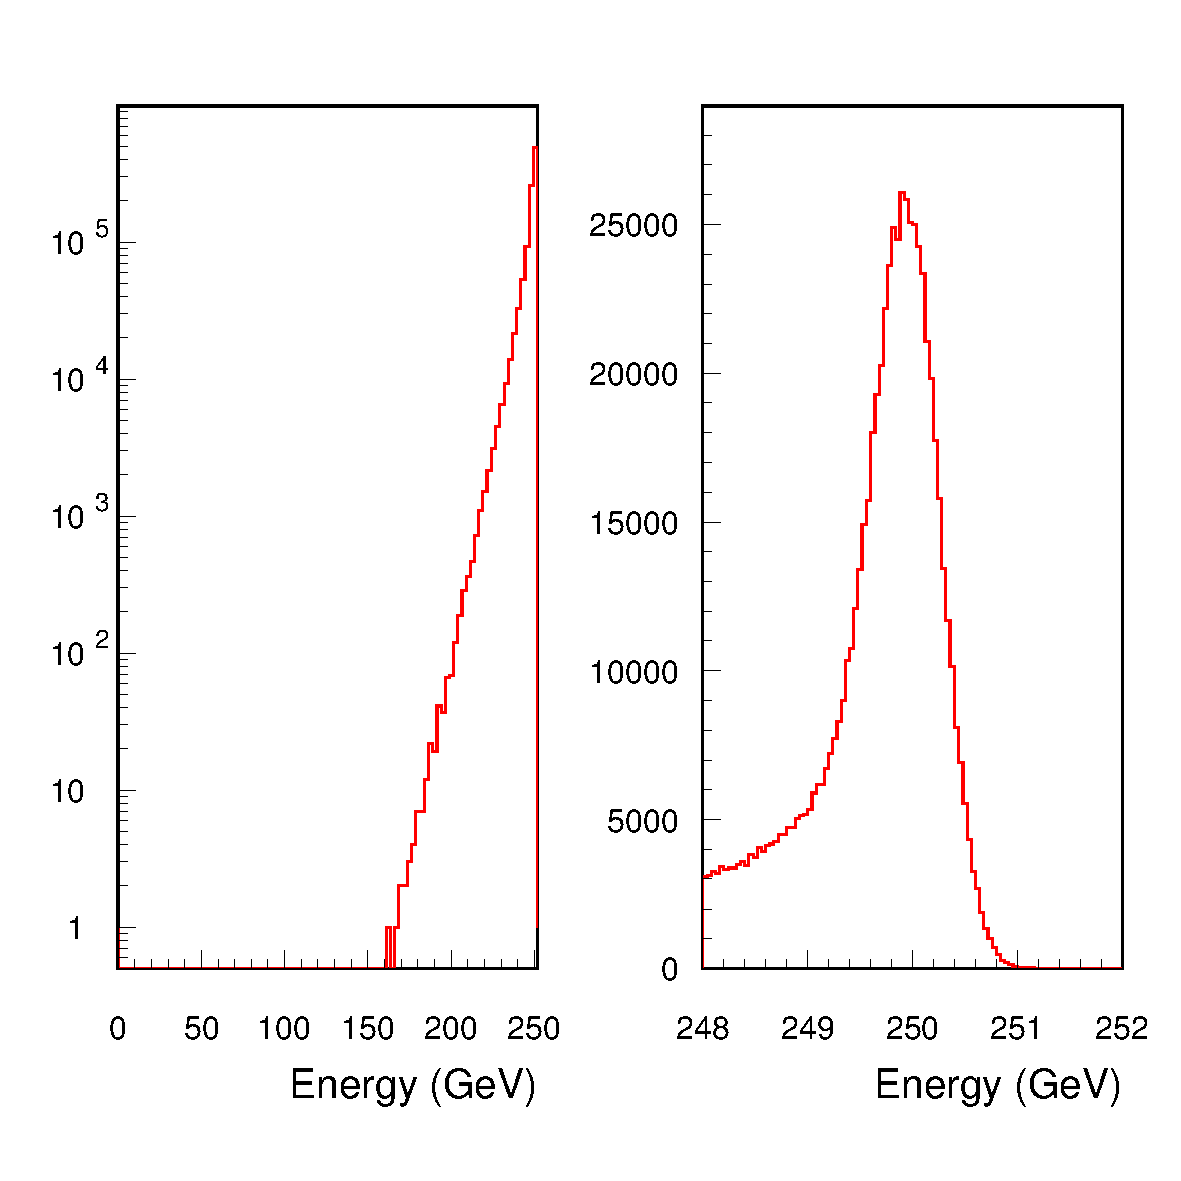
\includegraphics[width=\textwidth]{ILC/figs/ecmspect-250.pdf}
 \caption{ \label{fig:ilc:ecmspect-250}}
 \end{subfigure}
%\hspace{0.03\textwidth}
\begin{subfigure}{0.49\hsize} 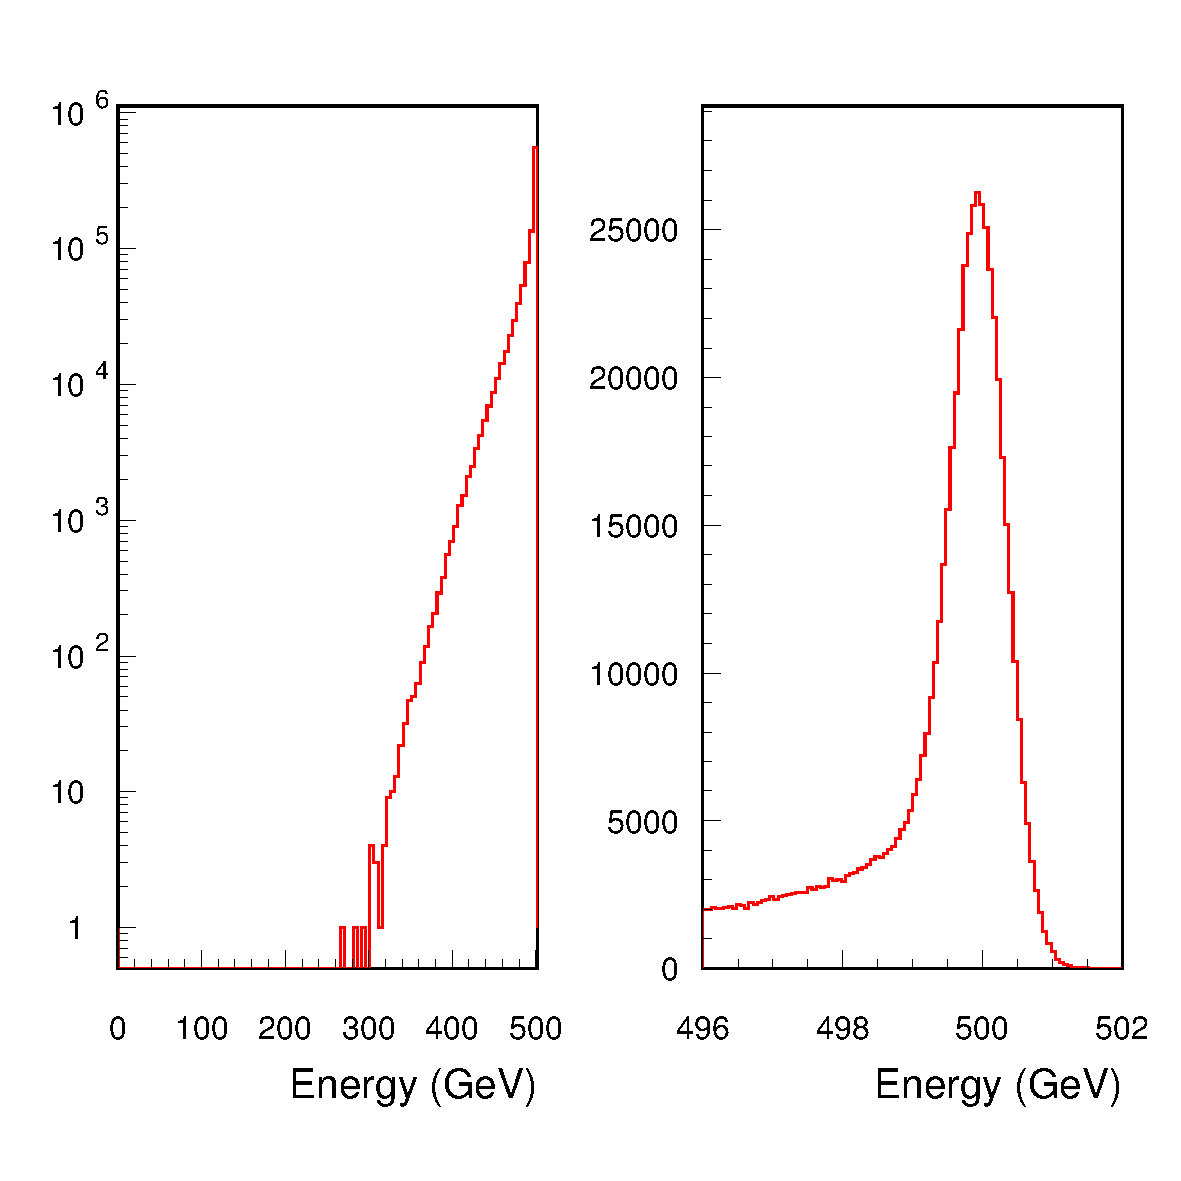
\includegraphics[width=\textwidth]{ILC/figs/ecmspect-500.pdf}
 \caption{  \label{fig:ilc:ecmspect-500}}
 \end{subfigure}
%\end{center}
\caption{
(a) Luminosity spectrum for ILC-250.
(b) Luminosity spectrum for the 500~\GeV~upgrade machine.
Spectra are generated with Guinea Pig (see section~\ref{sec:generator}).
}
\label{fig:ilc:ecmspect}
\end{figure}

The ILC beams produce three main sources of background in the detectors. Upstream of the collision region, the interaction of the electron and positron bunches with beam-line elements such as collimators produce high-energy highly penetrating muons parallel to the beam. Recent work has shown that the level of muon background can be reduced to a level tolerable for the detector \cite{Keller:2019aak}, with a hit occupancy well below the critical limits. 

%(\textit{exact meaning and value to be checked}). 
In the collision region, the strongly focused beams emit beamstrahlung photons in the very forward directions which leave the detector towards the main beam dumps. Secondary electron and positron pairs stemming from photon conversions and interactions are a source of backgrounds especially for detectors close to the beampipe. Finally, the neutrons produced in the main beam dumps 300\,m downstream of the interaction region can travel back into the detector. The three sources have been studied in detail and are under control~(see~section~\ref{ild:sec:beam_backgrounds}).

\subsection{Machine Detector Interface}
The requirements of a linear collider have technical implications for the ILD detector. All those aspects are summarised in the Machine-Detector Interface that has been specified and designed in close collaboration with the ILC machine groups and SiD~\cite{bib:sid:loi}, the other currently proposed detector for the ILC.

\subsubsection{Push-Pull}
The ILC is proposed to have a common Beam Delivery System that serves one interaction point shared between two detectors, ILD and SiD, that operate in a push-pull scheme~\cite{Behnke:2013xla}. In such a scheme, one detector is taking data on the ILC beam, while the other one is parked close by and waits for its turn to move in. Figure~\ref{ild:fig:push_pull} shows a conceptual design of ILD and SiD in such a push-pull configuration where both detectors are mounted on movable concrete platforms. The system is designed for short turn-around times of one day or less.
\begin{figure}[h!]
\centering
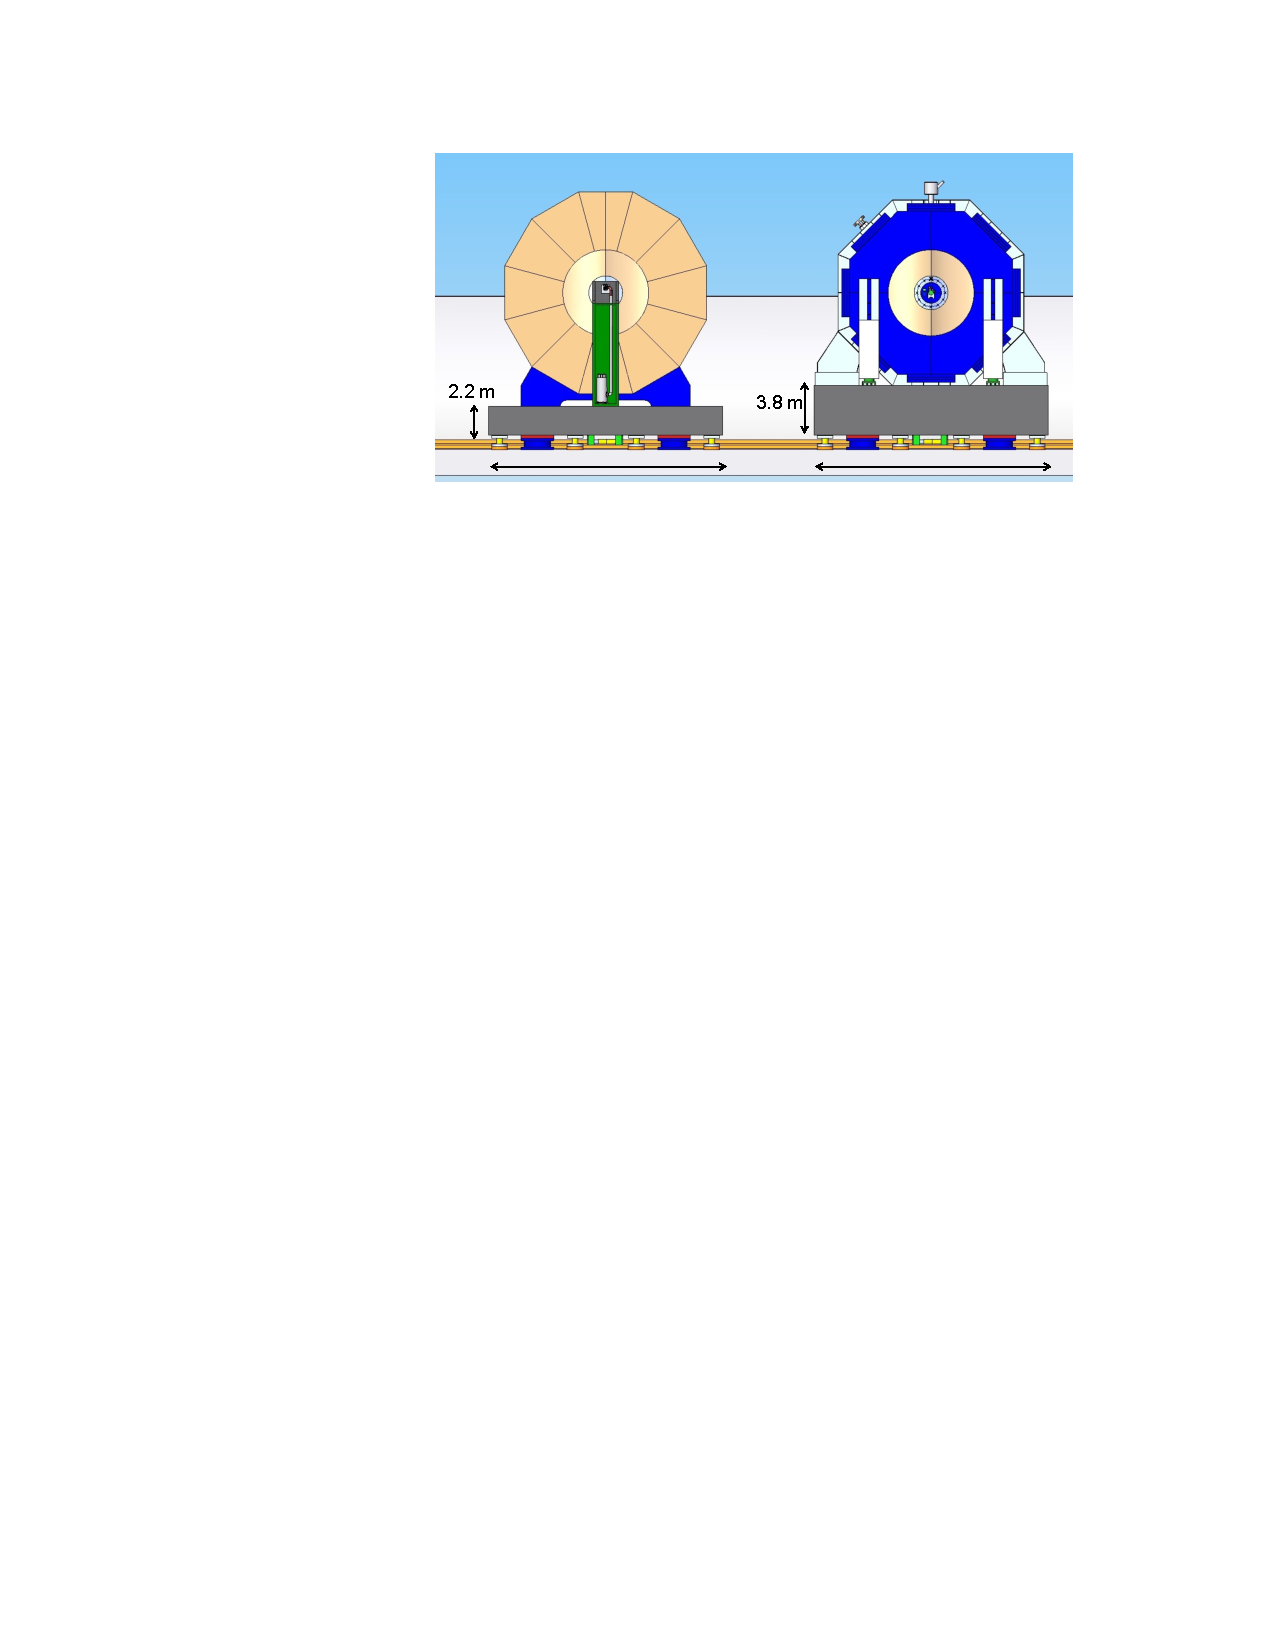
\includegraphics[width=0.8\hsize]{ILC/figs/push-pull.pdf}
\caption{\label{ild:fig:push_pull}Conceptual design of the push-pull system for ILD (left) and SiD (right). Both detectors are mounted on movable concrete platforms~\cite{Behnke:2013xla}.}
\end{figure}
The requirements for such a push-pull operation scheme have been defined between both detector collaborations~\cite{Parker:2009zz}. The impact of these requirements on the ILD design is discussed in more detail in section~\ref{ild:sec:external_integration}.

\subsubsection{Accelerator Elements}
The final focus magnets of the ILC are at a close focal length so that they have to be accommodated by the detectors. The closest magnet to the interaction point, the QD0 quadrupole, is an integral part of ILD, as can be seen in figures~\ref{ild:fig:Forward_QD0} and~\ref{fig:det:quad}. The QD0 magnet packages move together with the detector in case of push-pull operations, i.e. SiD and ILD both have their own set of magnets.
\begin{figure}[h!]
\centering
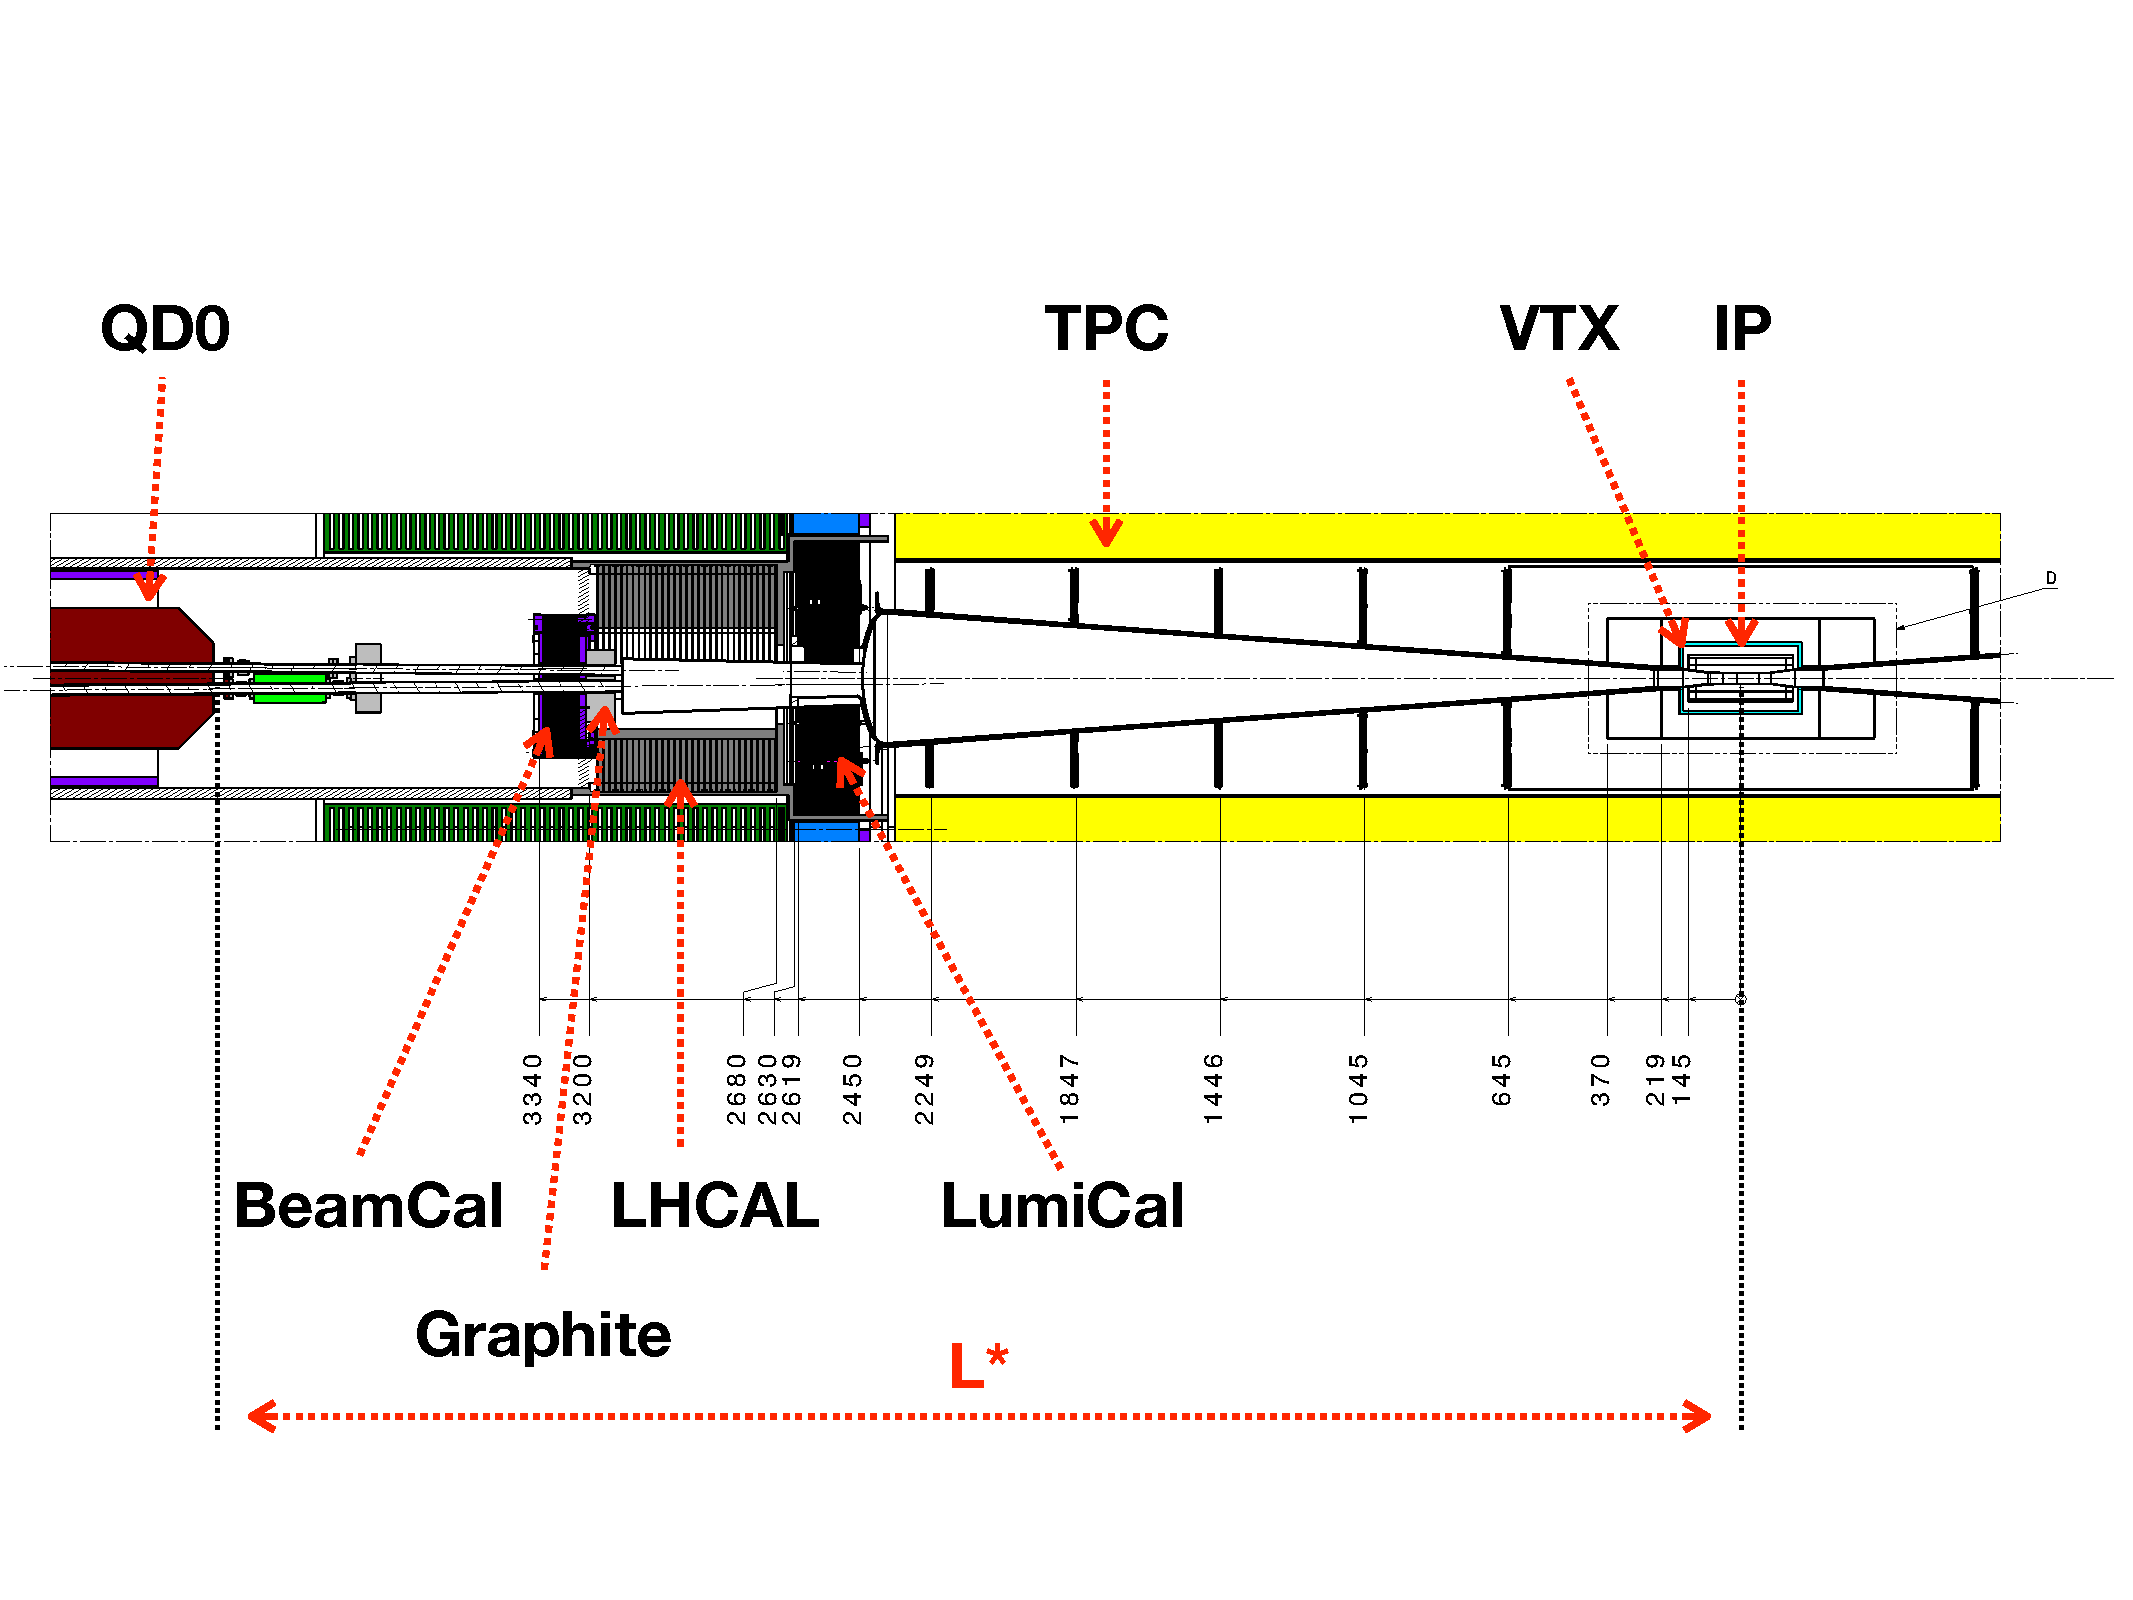
\includegraphics[width=0.8\hsize]{ILC/figs/ILD_Forward_Region.pdf}
\caption{\label{ild:fig:Forward_QD0}ILD forward region. The focal length $L^*$ in this design is 4.1 m. The interaction point IP is on the right of the picture, the main elements of the forward system are indicated in the drawing.}
\end{figure}
In the ILC TDR, two focal lenghts of the QD0 magnets were foreseen, 4.4~m for ILD and 3.5~m for SiD~\cite{Behnke:2013xla}. Later, the design of the ILC has been changed and the focal lengths were harmonised at 4.1~m~\cite{ild:bib:lstar_cr}. For ILD, this required a re-design of the forward region, since the QD0 magnet has moved closer to the interaction point, while the detector dimension remained unchanged. A vacuum pump located close to the interaction point had to be removed to provide the required space for the change. The pump removal was expected to deteriorate the vacuum levels in the central beam pipe of ILD. However, a study of the possible impact on backgrounds from beam-gas reactions showed that the estimated levels are still negligible~\cite{ild:bib:beam_gas}.
